\documentclass{report}
\usepackage{graphicx}
\usepackage{url}
\usepackage[utf8]{inputenc}

\title{2D Charts and their application to 3D}
\author{Sameer Al Harbi}

\begin{document}
\maketitle
\part{Charts and Analysis}
\today
\\
\begin{quote}
    The following is a compilation of 2D techniques to visualize data, after each a short analysis follows on the graphs suitability for expansion to 3D. There are naturally many other ways to plot data, but for the context of a limited project It was decided that the following would be chosen as Representative / first to be implemented if chosen for their respective family of data.
    
    But most importantly this document does not represent the end of research into new chart additions. There are multiple other charts that would become a great fit as the project progresses or some mentioned here that would become not as good of a fit. As such consider this as the initial, basic starting point for choosing a handful of graphs to start working on. 
\end{quote}
\\
\section{Pie Chart}
\begin{center}
    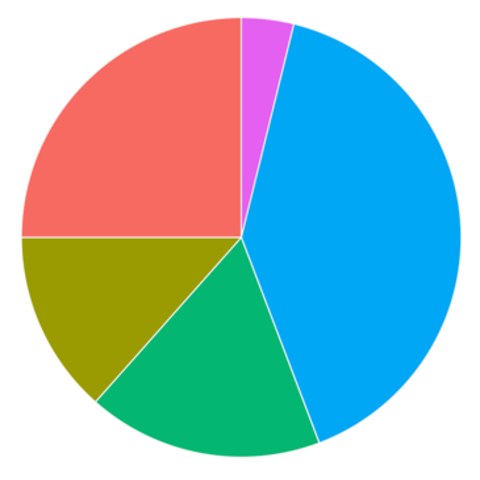
\includegraphics[width=150pt]{piechart-ggplot22.png}
\end{center}

The bar chart is a common chart that is used for showing how subsets of data fit into a whole. Market share of a product, etc.. One useful attribute that this chart can have is expanding it with a time or other similar dimension which can be represented as a video showing how each slice grows or shrinks as that dimension changes. A slider value to control this third dimension is a good idea. But otherwise this graph doesn't have any property that makes it uniquely suitable to 3D data and 3D visuals.


\section{Bar Chart}
\begin{center}
    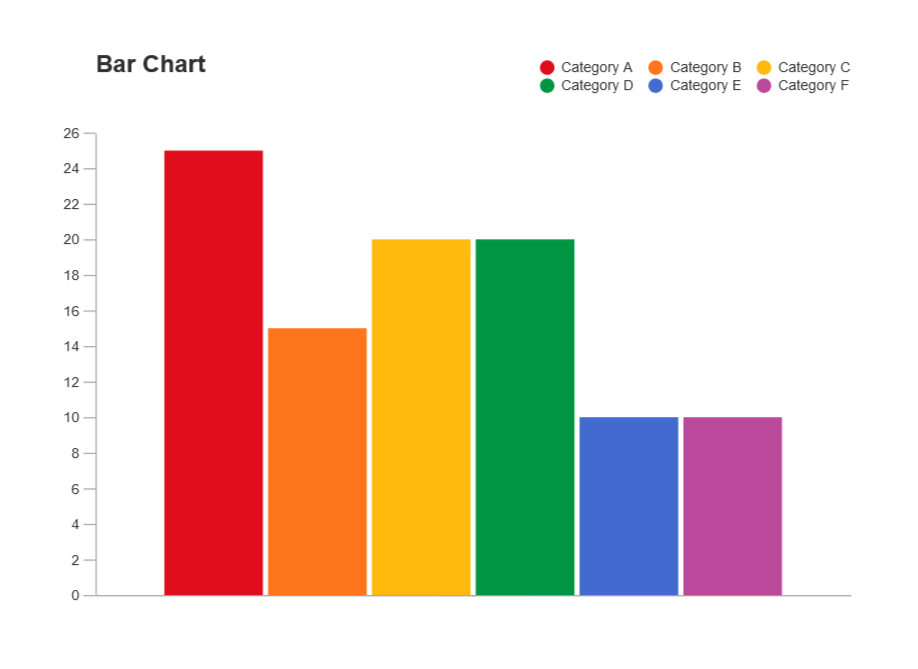
\includegraphics[width=150pt]{basic-bar-graph.png}
\end{center}

The bar chart is another very common chart that can be seen used for categorical or nominal data. Profit per year, etc..
3D charts can often be seen expanded into 3D over some third dimension showing multiple 2D charts side by side but the results are usually a little bit confusing. In that sense a slider like video could also work to clarify the visual from a UX standpoint. But otherwise this graph doesn't have any property that makes it uniquely suitable to 3D data and 3D visuals.

\section{Radar Chart}
\begin{center}
    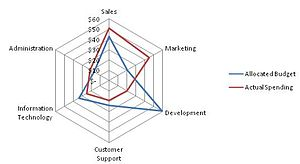
\includegraphics[width=150pt]{Spider_Chart2.jpg}
\end{center}

The Radar chart (or one of it's countless other names) is a chart that is used to display multivariate data i.e multidimensional data. In that sense it is a perfect chart to represent for this project as is and can most likely be represented in 3D quite easily by making use of the z axis instead of only relying on the x and y as 2D representations do.

\section{Scatter Plot}
\begin{center}
    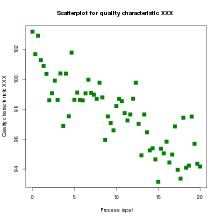
\includegraphics[width=150pt]{Scatter_diagram_for_quality_characteristic_XXX.svg.png}
\end{center}

The scatter chart is a very flexible chart that works by plotting points (such as measurements) over some, usually 2 dimensions to identify possible relationships. If data collected has more than 2 attributes then it would be very easy to render these points in 3D space such that it corresponds to each axis / attribute / dimension. 

\section{Box Plot}
\begin{center}
    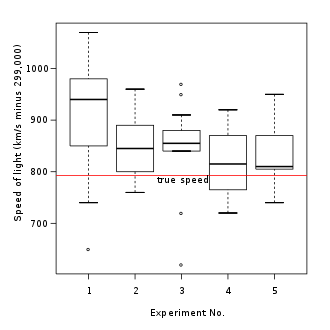
\includegraphics[width=150pt]{330px-Michelsonmorley-boxplot.svg.png}
\end{center}

Box plots are a way to visually show skewness and spread of numerical data. The multiple attributes that make up a box plot hint at a possibility of showing this data in a unique way in 3D and with more dimensions but at the moment nothing has been identified other than the method similar to 3D bar charts. This graph doesn't have any property that makes it uniquely suitable to 3D data and 3D visuals (that has been yet identified during the course of this project).

\section{Line Charts}
\begin{center}
    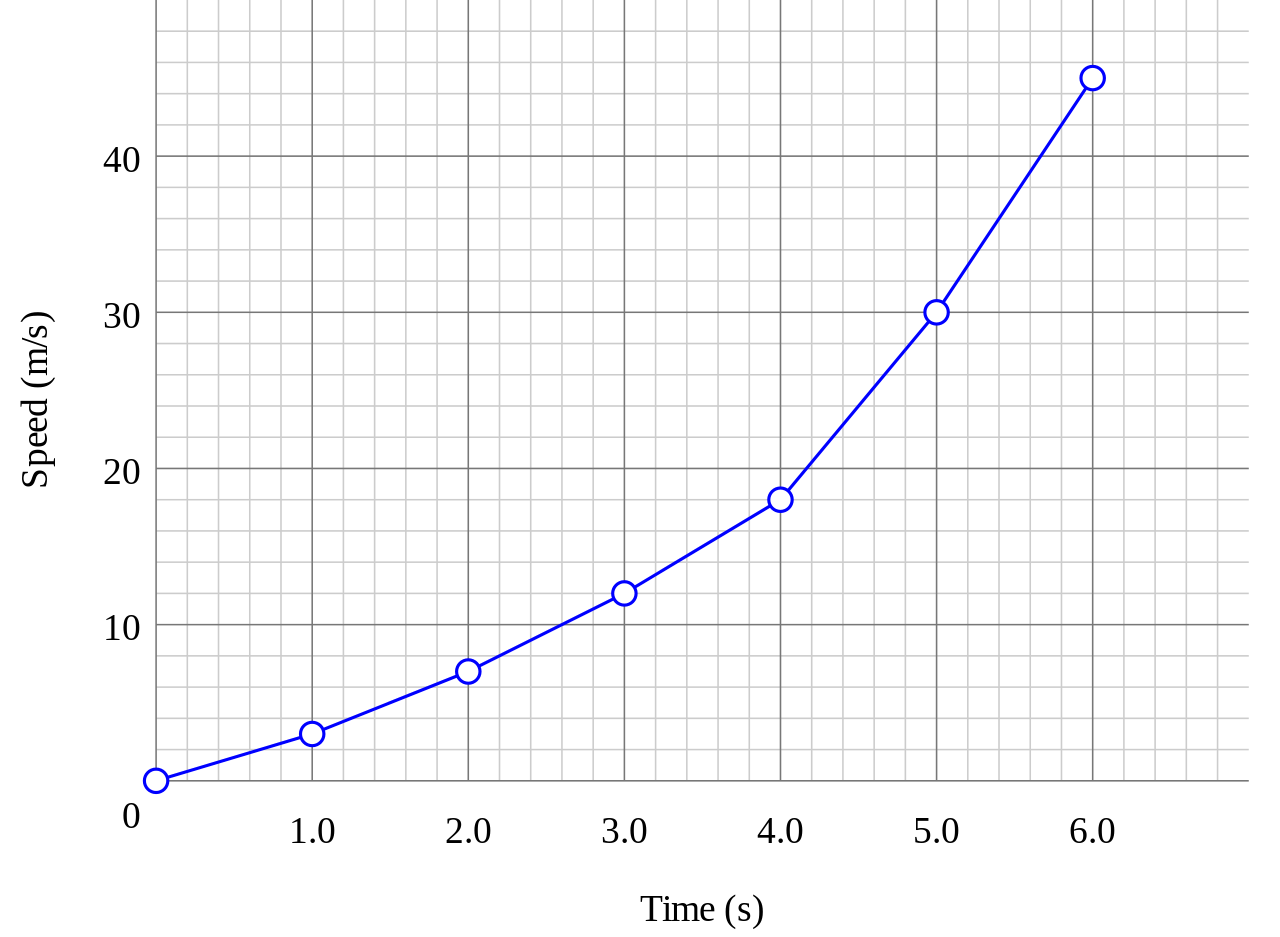
\includegraphics[width=150pt]{ScientificGraphSpeedVsTime.svg.png}
\end{center}

Line charts are a chart that shows information as interconnected data points on usually two axes. It would make sense that an extension to 3D and the use of the z axis as a third attribute would be a natural extension to this type of graph- but it is not clear how useful or accurate such a graph would be. This is a point that would need extensive research and would probably extend beyond the scope of this project. But otherwise this graph doesn't have any property that makes it uniquely suitable to 3D data and 3D visuals.

\part{Conclusions}

After considering 2D visualisations techniques and the data that is plotted with these techniques- I have identified some data types and visuals that would be both feasible and provide the most value when considering the creation of a 3D Data Visualisation program. These are:

\begin{enumerate}
    \item \textbf{Scatter Plot} is the best chart to out of all considered in this document to create a 3D visualiser for. The data is simple and essentially can be represented as coordinates in 3D space (The data is perfect for both creating 3D visuals and representing multidimensional data, another positive for the scatter plot). Visuals are also simple, just a dot at the correct coordinates. These two points make this graph a perfect first graph to get working as a test of the underlying system to correctly plot data- with all other graphs implemented afterwards using the foundation set here. 
    
    One further class of graphs to look into would be ones that model correlation data (Scatter plots fall into this category) as this kind of data seems to translate quite well when more attributes are added and a 3D render created.
    
    \item \textbf{Radar Chart} The radar chart is another graph that works well for multidimensional data and mostly translates visually to 3D. Rendering an understandable view might be troublesome so this chart takes the second place in priority
    
    \item \textbf{Dimensional Scale with all other graphs} The rest of the graphs such as the bar chart and pie chart all consist of data that cannot have another dimension added to them without disrupting the structure of the chart too much both when creating a 2D or 3D visual. A simple solution is creating multiple 2D views for each third and beyond dimension / attribute and allowing the user to use a scaling bar or other UX scheme to scroll through. This is not as intuitive and doesn't provide the advantages that the application hopes to bring as it does with the charts mentioned in previous points. As such, these charts that would use a "Dimensional Scale" are set as the lowest priority.
\end{enumerate}




\end{document}


